\documentclass[../../main.tex]{subfiles}

\begin{document}
Para empezar, un aspecto a notar sobre nuestros datos es que contienen características
temporales (la serie de tiempo univariada) y ``estáticas'' (el inicio de programa). Lo que
hicimos en todas las arquitecturas fue procesar la serie temporal por un lado y para hacer
la clasificación, combinar el resultado de este procesamiento con la entrada estática.

La salida de cada modelo es un número real que representa la probabilidad que la entrada
dada\footnote{En realidad, lo que producen las redes como salida es un valor real, y no
una probabilidad propiamente dicha. Para interpretar este valor como una probabilidad, se
debe aplicar una función sigmoide. Durante el entrenamiento, PyTorch provee una función de
pérdida llamada \texttt{BCEWithLogitsLoss}\cite{bcewithlogitsloss} que realiza
internamente esta ``conversión''.} - caracterizada por la serie de tiempo y el inicio de
programa - pertenezca a la categoría con etiqueta 1, que en nuestro caso representa formar
parte del grupo de control. Para obtener la clase final (0 o 1), se aplica (por fuera del
modelo propiamente dicho) un \textbf{umbral de decisión} sobre esta probabilidad: si la
probabilidad es mayor que dicho umbral, se considera que el modelo ha clasificado a la
entrada como pertenceciente a la clase 1. En este trabajo, fijamos este umbral en 0.5.

Dejamos algunos hiperparámetros fijos en todas los modelos:
\begin{itemize}[itemsep=0cm, topsep=0cm, parsep=0cm, partopsep=0cm]
    \item Número de épocas de entrenamiento: 100.
    \item Número de capas para el procesamiento de series temporales: 2.
    \item Optimizador: Adam.
\end{itemize}

Y aquellos sobre los que llevamos a cabo una búsqueda fueron los siguientes:
\begin{itemize}[itemsep=0cm, topsep=0cm, parsep=0cm, partopsep=0cm]
    \item Tamaño de lote: probamos con 32, 64 y 128.
    \item Número de neuronas por capa: probamos 32, 64 y 128.
    \item Tasa de aprendizaje: probamos con 0.01, 0.001 y 0.0001.
    \item Dropout: probamos con 0.3, 0.5 y 0.7.
\end{itemize}

Para hacer esta búsqueda, utilizamos la técnica de validación cruzada sobre los conjuntos
de entrenamiento con 3 particiones, cada una manteniendo las proporciones originales de 0s
y 1s del conjunto de entrenamiento. La métrica que se buscó optimizar fue el puntaje
\(F_1\) sobre la clase positiva - discutido posteriormente en la Sección
\ref{sec:metricas} - promediado sobre las tres iteraciones de la validación cruzada.

En lo que sigue, incluimos ilustraciones y detallamos en profundidad las arquitecturas
utilizadas. Para diseñarlas, tomamos como base las propuestas en
\cite{wang2016timeseriesclassificationscratch}, \cite{Karim_2018} y
\cite{timeseriesclass-with-rnn}.

\subsection{Arquitectura 1: Red LSTM}
Como se puede ver en la Figura \ref{fig:lstm_v2}, en la primera arquitectura propuesta, la
serie de tiempo es procesada por dos capas LSTM con una capa intermedia de dropout.
Posteriormente, se realiza una operación de concatenación, en la que se combina la salida
del ``bloque'' LSTM con la característica correspondiente al inicio del programa en un
vector unidimensional que puede ser ``alimentado'' a capas totalmente conectadas. De esta
forma, el vector se introduce en una red densa compuesta por una capa oculta de 128
neuronas con función de activación ReLU, seguida de una capa de dropout, y finaliza en una
capa de salida que produce la probabilidad final.
\begin{figure}[ht]
    \centering
    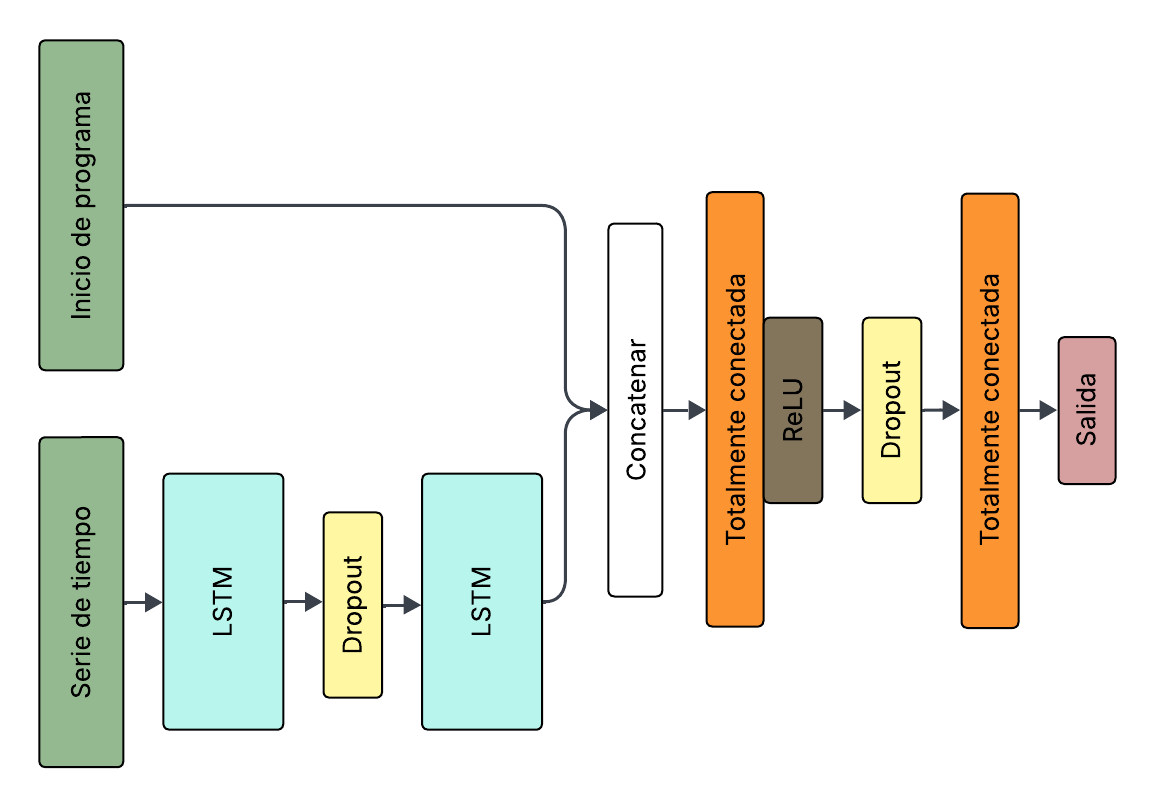
\includegraphics[width=0.6\textwidth]{figs/lstm_v2.png}
    \caption{Esquema de la arquitectura de la red LSTM propuesta.}
    \label{fig:lstm_v2}
\end{figure}

\subsection{Arquitectura 2: Red Convolucional}
El segundo modelo propuesto sigue la misma estructura general que la arquitectura
anterior, pero reemplazando las capas LSTM por capas convolucionales. Concretamente, ahora
el procesamiento de la serie temporal se realiza mediante dos capas convolucionales, cada
una con normalización de lote y ReLU, y entre medio de ellas una capa de dropout. A
continuación, se aplica una segunda capa de dropout y una operación de average pooling. La
primera capa convolucional aplica 128 filtros de tamaño 3 con padding, la segunda aplica
256 filtros de tamaño 2 sin padding, y el filtro del pooling es de tamaño 2. Finalmente,
la salida resultante se convierte en un vector unidimensional que es la entrada de las
capas posteriores del modelo, encargadas de finalizar la clasificación. La Figura
\ref{fig:conv} muestra un diagrama de esta arquitectura.
\begin{figure}[ht]
    \centering
    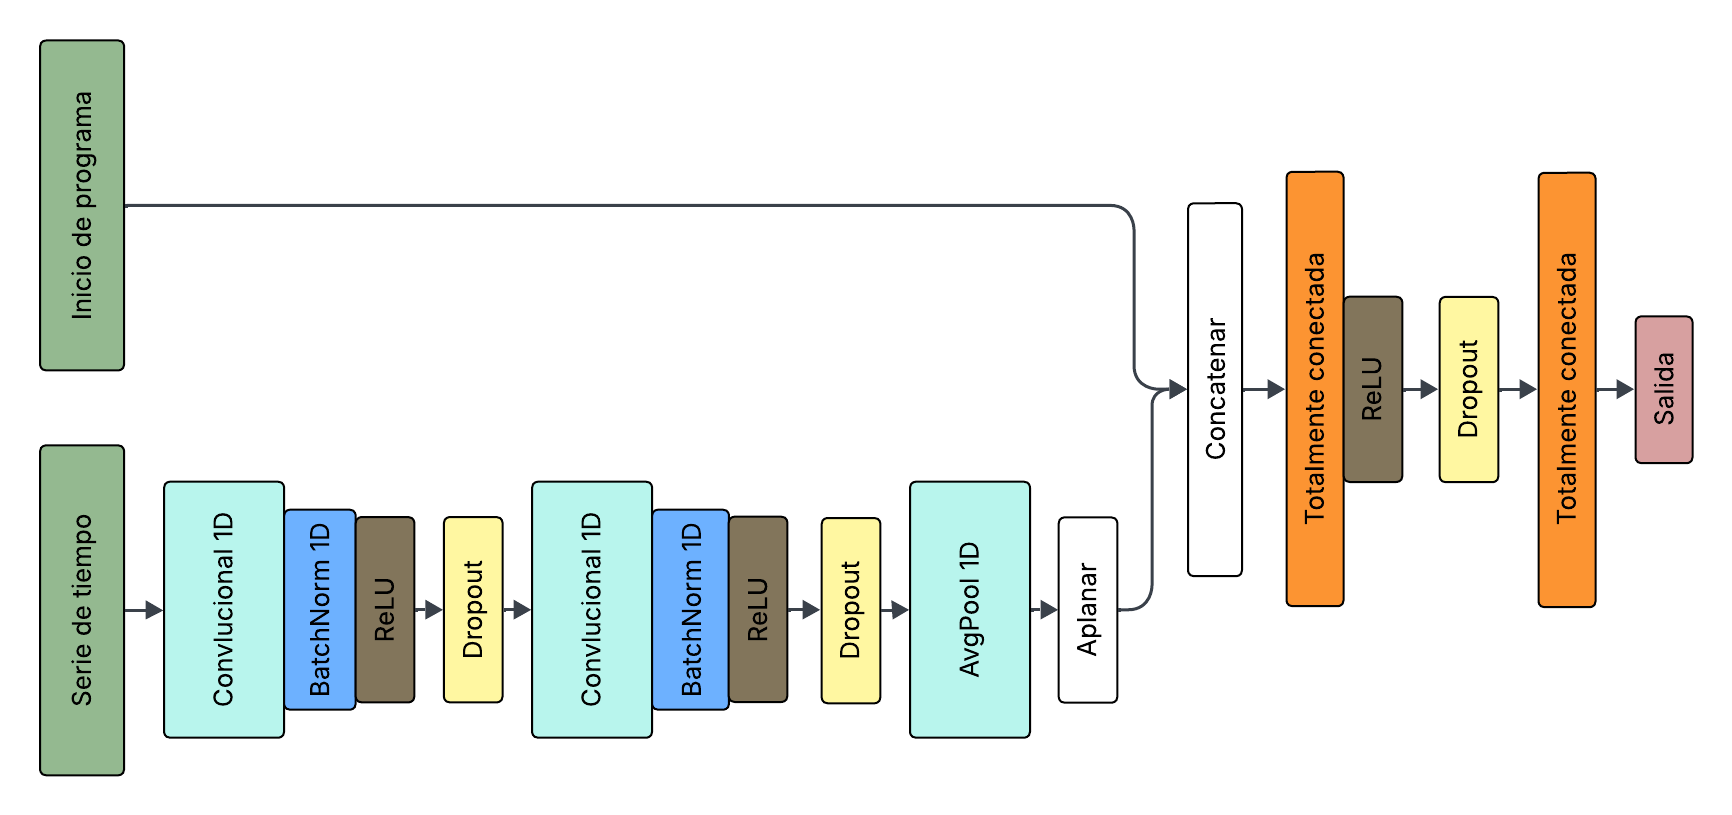
\includegraphics[width=0.8\textwidth]{figs/conv.png}
    \caption{Esquema de la arquitectura de la red convolucional propuesta.}
    \label{fig:conv}
\end{figure}

\subsection{Arquitectura 3: Red Convolucional + LSTM}
Esta última arquitectura combina las otras dos: ahora, el procesamiento de la serie
temporal es llevado a cabo de manera paralela por las capas LSTM de la Arquitectura 1
y las capas convolucionales de la Arquitectura 2. Luego, se combinan ambas salidas y
el inicio de programa para posteriormente producir la predicción final a través de la
red totalmente conectada. La Figura \ref{fig:lstm_v2_conv} muestra un diagrama de esta
arquitectura.

\begin{figure}[ht]
    \centering
    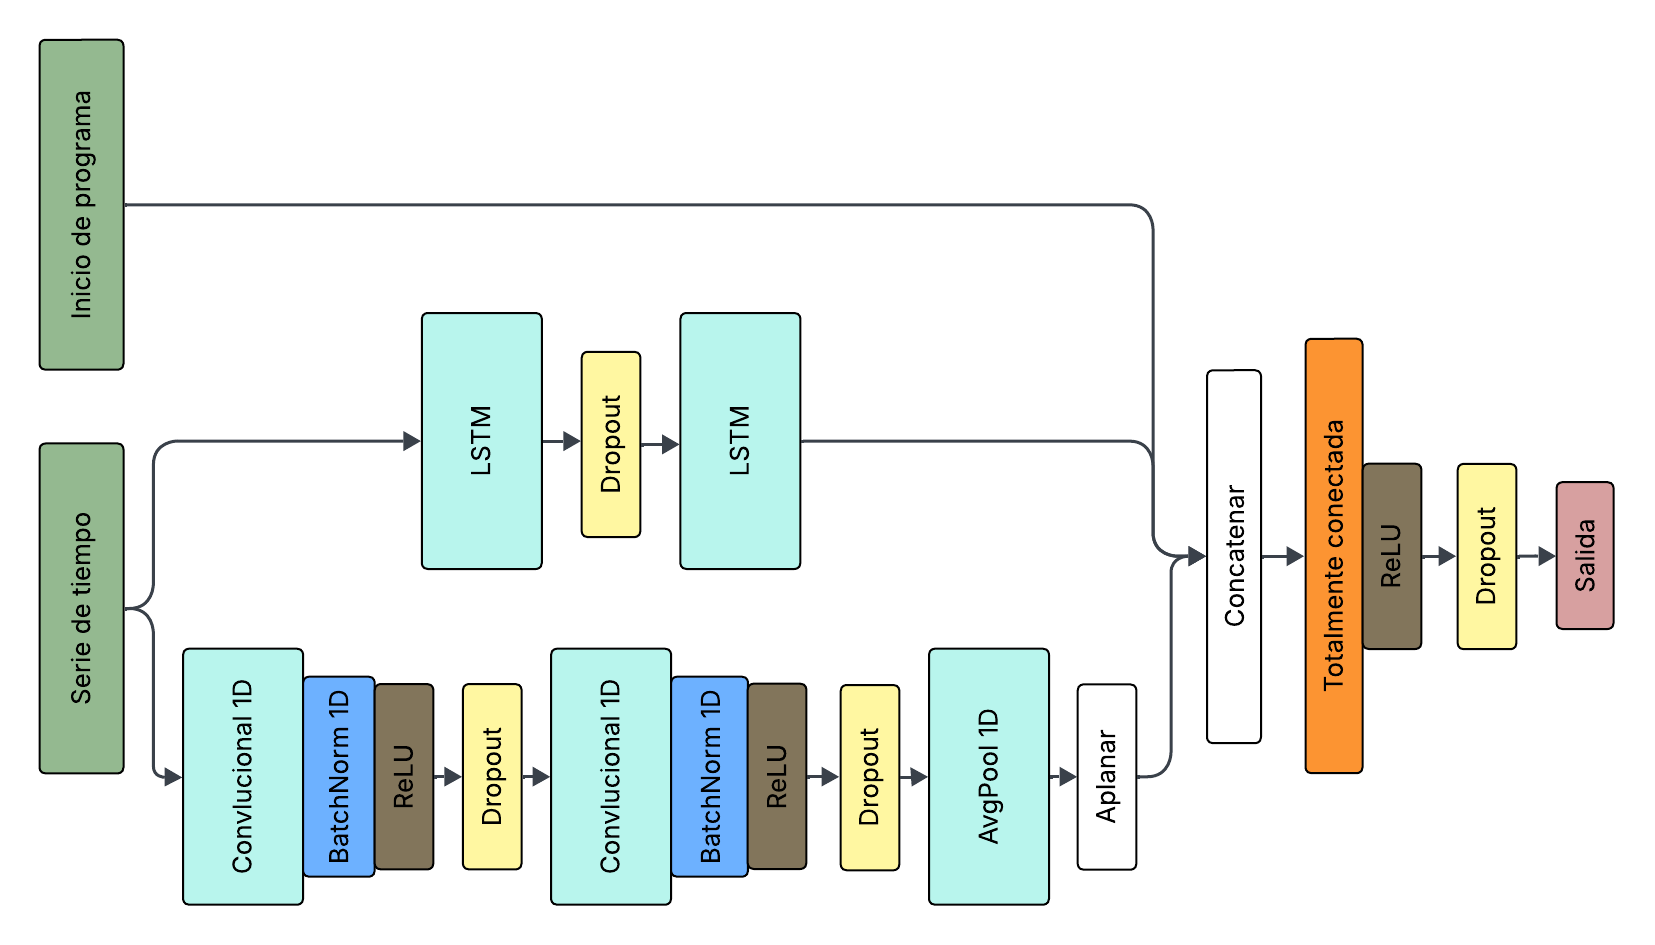
\includegraphics[width=0.8\textwidth]{figs/lstm_conv.png}
    \caption{Esquema de la arquitectura de la red LSTM + convolucional propuesta.}
    \label{fig:lstm_v2_conv}
\end{figure}

\end{document}